\chapter{Fundamentals and Related Work}
\label{chap:1}
%
\section{State of the Art}

\section{Probabilistic Estimation Methods}

TO DO

\section{Movement Prediction}

Foresee future moments and trajectories for dynamical objects in traffic scenarios is vital in order to obviate risks which occur on the roads. Prediction despite of short or long term they are, must have sufficient time in advance to avoid traffic situations we, as traffic participants, don't want. In this section, relevant researches for trajectory and movement predictions are introduced. \\

There is numerous research made on a trajectory and movement predictions with a vehicle as interest on traffic scenarios. \cite{ClassificationI} suggesting a one way of classifying methods for motion prediction. The main three categories with an increased rate of flexibility were defined: \textbf{\textit{physical-based, maneuver-based}} and \textbf{\textit{interaction aware}}.

\begin{itemize}
	\item \textbf{Physics-based} motion models are the most simple of all categories. It is considered that the movement of vehicles depends only on the laws of physics. A wider description is in subsection ~\ref{subsection:phb}.
	\item \textbf{Maneuver-based} motion models are more advanced than physics-based because maneuver-based motion models also consider future movements of a car which also depends on the maneuver which is intended to perform by a driver. A wider description is in subsection ~\ref{subsection:mb}.
	\item \textbf{Interaction-aware} motion models take into account consideration connections between maneuvers of the car, as well as rules of the traffic. This method as not so popular as previous ones due its complicity to adapt to the real life scenarios. A wider description is in subsection ~\ref{subsection:inaw}.
\end{itemize}

Figure~\ref{fig:MotModOv} summarizes motion models defined in \cite{ClassificationI}.

\begin{figure}[h]
	\centering  	
	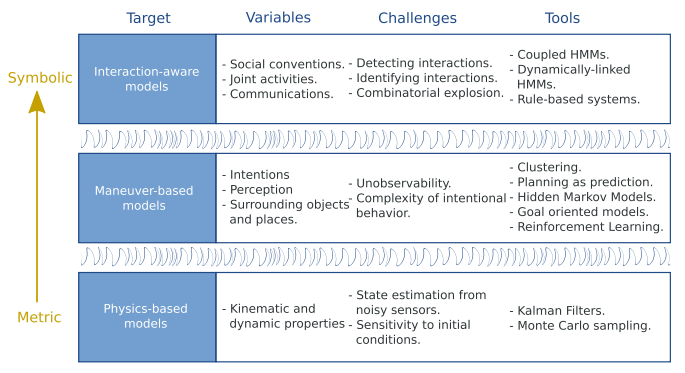
\includegraphics[width=15cm]{img/2.jpg}
	\caption{Motion Modeling Overview \cite{ClassificationI}}
	\label{fig:MotModOv}    
\end{figure}

Together with above-mentioned categories, authors of \cite{ClassificationII} introduced one more category to predict movements - \textbf{\textit{data-driven based}}.

\begin{itemize}
	\item \textbf{Data-driven} based motion and trajectory prediction can be classified into clustering-based and probabilistic approaches. A wider description is in subsection ~\ref{subsection:ddr}.
\end{itemize}

\subsection{Movement Prediction Using Physics-Based Models}
\label{subsection:phb}

Physics-based movement prediction models imply vehicles as a dynamic item, controlled by the physics' laws. Movements are predicted using dynamic and kinematic models with control inputs (e.g. acceleration, deceleration, steering), properties of the car (e.g. length, weight) and some external conditions (e.g. the friction coefficient of the road surface) to the process state of the vehicle (e.g. position, speed, direction). Great work has been done using \textit{physics-based} motion models and it still remains the most commonly used motion models for motion prediction in the context of road safety. The complexity of the models depends on a representation of the dynamics and kinematics of a vehicle, as well as, how uncertainties are handled, whether or not the road geometry is taken into account, etc. \\

Dynamic and kinematic models can be used for movement prediction in a lot of different ways, the main difference is how uncertainties are handled. Three main approaches will be described as follow: \textbf{\textit{single trajectory simulation, Gaussian noise simulation}} and \textbf{\textit{Monte Carlo simulation}} \cite{ClassificationI}.

\begin{itemize}
	\item \textbf{Single Trajectory Simulation.} The simplest method to predict future movements and trajectory of a car is to apply simple dynamic or/and kinematic models for the current state of a car while assuming that the current state of the car is determined with absolutely highest confidence and applied model (dynamic, kinematic or both) is the perfect representation for the movement of the car. This simple approach was used in \cite{dynamic} using dynamic and \cite{kinematicI, kinematicII} kinematic models. The main benefit of this straightforward approach is computational efficiency, that allows this method to be used in real time. On the other hand, predictions made by this method do not consider uncertainties of the current state and as a result, predicted movements and trajectories are not trustworthy for use in a long term ( > 1 sec.) predictions.
	\item \textbf{Gaussian Noise Simulation.} The uncertainty of the current state of a vehicle and its evolution during the time is a very important factor in movement or trajectory prediction and it can't be avoided. In \cite{GaussianNoiseI, GaussianNoiseII, kinematicII} this is modelled using a normal distribution. Gaussian Noise function is very popular because of its uncertainty representation in \gls{KF}, which is still a conventional method for vehicle state estimation having noisy sensors measurements in account. There are some cases where dynamic, kinematic and sensor models are linear and uncertainty is modelled using a normal distribution instead of \gls{KF} Bayesian filter is used. Filtering mainly contains of two steps: prediction and update steps. In the first time step at time step t, a current state of the vehicle is is given to the dynamic or kinematic model, which gives predicted state for the next time step which has a Gaussian distribution shape. In the following step, predicted state of the next time step is combined with sensor measurements of the same time step, which is Gaussian distribution as well. Filtering is a looping of these two steps every time when new measurements are available.
	
	By looping the first step, it is possible to get a mean and covariance matrix for every future timestep for the vehicle state. This can be modified into a trajectory mean with linked uncertainty (i.e. normal distribution in each timestep), as showed in \cite{GaussianNoiseIII, GaussianNoiseI}. As compared to the approached of \textit{single trajectory simulation}, Gaussian Noise simulation techniques have the benefit of uncertainty representation on the predicted trajectory or movements. However, there are some limitaitons as well: modelling uncertainties employing normal distribution is not quite enough to show the different possible maneuvers. A possible solution for this could be uncertainty representation using \gls{VGMM}. Author of \cite{SKFI} used \gls{SKF} for this exact purpose. \cite{GaussianNoiseII} depends on mass of \gls{KF} to show possible models for movement evolution for vehicle and be able to freely change between them. \cite{kinematicII} introduced an alternative approach: to use heuristics and change different kinematic model depending on the current situation.
	
	\item \textbf{Monte Carlo Simulation.} In generic case  when no assumptions in advance are made about models linearity or uncertainty model, distribution expresion on predicted vehicle states are not clear. Monte Carlo method is the right tool for this kind of situation. The idea under the Monte Carlo method is to randomly sample the input of the dynamic or kinematic model and to generate potential future trajectories. If the road topology is taken into account, various mass can be added to the generated trajectories and movements to penalize the ones which do not respect the restriction of the road design. Kinematic and dynamic models can be used for Monte Carlo method by categorizing inputs instead of considering them as a constant. Typical inputs are categorized to acceleration, steering angle or lateral deviation. To be able to take into account eligibility of the movement, generated trajectory samples, which has a bigger acceleration than physically is allowed can be removed, as it was done in \cite{MonteCarlo} or consider limitations which vehicle has (weight, length, etc.) and distribute dynamic and kinematic models in a more realistic manner and remove all impracticable trajectories from predefined trajectories list as it was done in \cite{MonteCarloI}. Monte Carlo method can be used to foresee trajectory or movements for a vehicle with a very well known current state or for vehicle which has uncertainty in the current state, which was estimated by one of the filtering algorithms.
\end{itemize}

\subsection{Movement Prediction Using Maneuver-Based Models}
\label{subsection:mb}

\textit{Maneuver-based} motion models show vehicles as independent moving entities, i.e. it is assumed that the movement of a vehicle on the road match to a series of independently executed movements from the other vehicles on the same road. Oxford dictionary \cite{def} a movement/maneuver as “a physical movement or series of moves requiring skill and care”. Term behaviour in literature often is used meaning the same meaning, e.g. in \cite{beh1, beh2, beh3}, for the sake of simplicity word "movement" or "maneuver" will be used in this work with defined meaning. Movement and trajectory prediction using maneuver-based motion models work with in advance recognized movements which driver possibly intend to perform. If an algorithm can recognize intended movement, the algorithm can assume that future actions of the driver will match the recognized movement. Due to this a \textit{priori} information, trajectories received with this method are more relevant and reliable than the ones received using physics-based motion models.  Maneuver-based motion models rely on prototype trajectories or on movement intention estimation. \\

Vehicle motion classification into maneuver/movement classes has been extremely widely applied not only in driver assistance systems but into natural driving studies \cite{DataDrivenIV, DataDrivenV, DataDrivenVI, mab1, mab2, mab3, mab4, mab5, mab6, mab7}. Authors of the majority of approaches are using heuristinc \cite{mab1} or training classifiers like \glspl{SVM} in \cite{mab2}, \glspl{HMM} \cite{DataDrivenIV, mab3, mab4}. \glspl{LSTM} in \cite{mab5}, Bayesian networks \cite{mab6}, etc., as movement-based features using speed, deceleration, acceleration, yaw rate, lane position, turn signals, distance from other vehicle and other road context information. Authors of \cite{mab1} classified vehicle's movement into class "keep lane" or "change lane" grounded on how far the closest car is and predicted future trajectory by applying quintic polynomial of the current car movement state and pre-defined ultimate movement state for each movement class, defined before.Authors of \cite{mab6} used six different movement classes, which were defined before and using \gls{DBN} based on multiple movements and context based features selected the potentially right future movement. Authors of \cite{mab7} defined an individual Gaussian process for three movement classes and established a multi-modal distribution for possible future trajectories using each model. However, in the study, only one case-based prediction has been introduced. Authors of \cite{DataDrivenIV} also determined separate Gaussian processes, this time for four different movement classes, which were classified using a hierarchical \gls{HMM}. This method was tested on real highway data. Authors of another study \cite{DataDrivenV} used a random forest classifier for movements classification into pre-defined movement classes: left or right lane changes or keep lane. Authors used a separate \gls{GMR} model for predicting lateral movement for vehicles using each class. Method was tested on real highway data. Similar method, but without predifined movements classes for prediction longitudinal motion for vehicles were used in \cite{DataDrivenVI}.

\subsection{Movement Prediction Using Intention Aware Models}
\label{subsection:inaw}

\textit{Interaction-aware} motion models introduce cars as
manoeuvring items which co-operate with each other, i.e. a movement of a vehicle is considered to be affected by a movement of the other moving object in the traffic scene. Keeping into account the dependencies between the separate moving objects leads to a much better explanation of their movement compared with \textbf{maneuver-based} motion models described in the previous subsection.  As a result, it gives a better perception of the current situation. \\

Despite this, a relatively small amount of researches is done considering inter-moving-objects interaction in movement prediction. Authors of \cite{InterAwareI} assigned two movement classes for vehicles approaching an intersection together, applying a polynomial classifier which "punishes" cases that potentially would lead to near-collisions situations. Authors of \cite{InterAwareII} worked with a much complex scenario and assigned movement classes to multiple together interacting vehicles in a highway scenario. However, foreseen movements, trajectories of a vehicle are assumed to be given in advance. Results reported using a simulated environment. \cite{ClassificationII} in their work considered multiple interacting vehicles together with the difficulty of estimating their future motion.  Authors of \cite{DataDrivenV} not directly used inter-moving-objects interaction by including comparative positions and velocities of vehicles close by as features for movement and trajectory prediction.

\subsection{Movement Prediction Using Data-Driven Model}
\label{subsection:ddr}

As mentioned earlier \textit{data-driven} movement prediction can be generally classified into clustering-based and probabilistic approaches.  \textbf{Clustering-based} approaches group the training data in order to provide a set of possible prototype trajectories \cite{DataDrivenI, DataDrivenII}. Partially observed trajectories are checked and compared with a prototype trajectory using various distance measurements, as \gls{DTW}, \gls{LCSS}, Hausdorff distance, etc. and after matching movement trajectory with prototype trajectory, later one is used as a model for future movement. Clustering approach is quite easy, but the main disadvantage of this method is the deterministic nature of the predictions. \\

\textbf{Probabilistic} approach contrary learn probability distribution of every movement trajectory class and gives the conditional distribution for future movements, given current trajectory. This lets us avoid some degree of natural uncertainty of predicting the future. \\

Authors of \cite{DataDrivenIII, DataDrivenIV} for modelling trajectories and for motion prediction use Gaussian Processes which are the most popular approaches solving prediction problems so far. \cite{DataDrivenV} uses \gls{GMR} for prediction longitudinal movement of a vehicle, while \cite{DataDrivenVI} uses the same method for lateral movement prediction. \cite{DataDrivenVII} uses \glspl{VGMM} for conditional distribution within snippets of future having snippets of movement history models. The latest approach is much easier and computationally more effective when compared to Gaussian Process Regression.  Authors proved the efficiency of method predicting non-linear movements in turns at the intersection scenarios. 

\subsection{Limitations of Methods for Movement Prediction}

Subsections~\ref{subsection:phb},~\ref{subsection:mb},~\ref{subsection:inaw} and~\ref{subsection:ddr} described movement prediction with different feature based model. This subsection will introduce limitations of all these methods.

\begin{itemize}
	\item \textbf{Physics-based approach.} Predictions using physics-based motion models are restricted to very short-term ( < $1$ sec.) motion prediction due to low-level motion (dynamic and kinematic) properties this method relies on. Usually using this method it is  unable to foresee any change in the vehicle movement which happens due to an execution of a particular maneuver (e.g. speed up, slow down, make a turn, etc.), or changes caused by external factors (e.g. slowing down due to traffic lights, signs, other vehicles, etc).
	
	\item \textbf{Maneuver-based approach.} For a very long time, the biggest limitation of prototype trajectories was time representation. When the movement models are showed using a finite set of trajectories it takes a very large number of prototypes to represent the large variation
	in the implementation of an every possible movement pattern. Handling subtle situation in traffic, as movements with waiting time at a stop line, not constant velocity caused by traffic is a very big issue for such models. For a certain extent, \gls{GP} were introduced. They solved this kind of problem by introducing time-independent movement patterns \cite{DataDrivenIII}. On the other hand, \glspl{GP} have some other limitations as well. First of all to be able to take into account all possible traffic scenarios, has very heavy computational time, despite that they are not considering the physical limitations of a vehicle and due to that may generate or predict unrealistic trajectories and movements. To solve these problems the best solution so far was proposed in \cite{RRT}. Authors used \gls{RRT} to be abe to "randomly sample points toward dynamically feasible trajectories, using as inputs the current state of the vehicle and the sample trajectories generated by the \glspl{GP}"  \cite{RRT}. Another issue with using predefined prototype trajectories is an adaptation to a different road, i.e. for different intersections. Each movement model is defined for a specific road/intersection geometry and topology, what means that prototype models only can be used with the same or very similar topology. 
	
	Maneuver-based approach contains similar limitations which described under limitations of data-driven approach.
	
	\item \textbf{Interaction-aware approach.} Prediction using interaction-aware motion models are the most exhaustive method suggested in the literature so far. Using it, is possible to predict for a longer-term as compared to physics-based motion prediction models, and predictions are more trustworthy than using maneuver-based motion models in predictions due to taking dependencies between the surrounding cars into consideration. However this completeness has some disadvantages as well:  calculation of all possible trajectories with all possible models take a lot of time and because of that, it is not very compatible with using in real-time situations. For this reason, using interaction-aware motion predictions are not so popular. 
	
	\item \textbf{Data-driven approach.} The assumption that movement of vehicles do not depend on each other and other traffic participants is not accurate.  All vehicles without any exceptions use a road together with other traffic participants and movement performed by one vehicle directly or indirectly effects others. Dependencies with each other are quite strong at intersection, where road rules, not only movement of other cars must be taken into account. Ignoring these reliances can lead to wrong interpretations of the situations, and affects the evaluation of the risk. A data-driven approach is quite easy, but not always it pays attention to these critical dependabilities and it is quite difficult to pre-define all possible action of other traffic participants, i.e. the main disadvantage of this method is the deterministic nature of the predictions.
\end{itemize}